In this section the compact models presented in chapter \ref{chapter:compact-models} are evaluated focusing in particular on MTZ and its variants and and GG models. To test them, a set of 20 instance of 50 nodes was generated and  was runned with a global timelimit of 30 minutes. The results are visible in figure \ref{fig:result-compact}.

\begin{figure}[h]
	\centering
	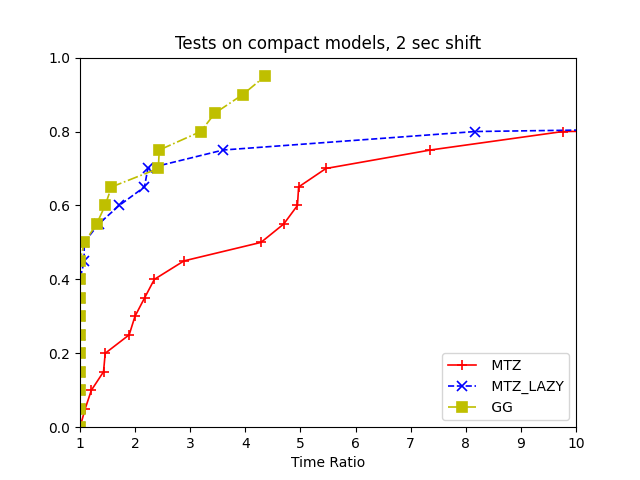
\includegraphics[width=0.6\textwidth]{images/final_mtz_mtzlazy_gg.png}
	\caption{The comparison chart of the compact models.}
	\label{fig:result-compact}
\end{figure}

From this image, it can be stated that the MTZ basic model is far from being the best one, and the best models are GG and MTZ\_LAZY - which perform in a comparable way. However, it is possible to see the that GG model deliver a consistent solution of the instance, while MTZ\_LAZY has reached the timelimit in some cases.